\section*{Часто используемые ядра \(K(r)\)}

\begin{figure}[h]
    \centering
    \includegraphics[width=\textwidth]{chapters/metric/images/I1.png}
    \caption{Графики ядер}
    \label{fig:kernels}
\end{figure}

\begin{align*}
\Pi(r) &= [{\lvert r \rvert \leq 1}] \quad \text{— прямоугольное} \\
T(r) &= (1 - \lvert r \rvert) [{\lvert r \rvert \leq 1}] \quad \text{— треугольное} \\
E(r) &= (1 - r^2) [{\lvert r \rvert \leq 1}] \quad \text{— квадратичное (Епанечникова)} \\
Q(r) &= (1 - r^2)^2 [{\lvert r \rvert \leq 1}] \quad \text{— квартическое} \\
G(r) &= \exp(-2r^2) \quad \text{— гауссовское}
\end{align*}


\section*{Выбор ядра \(K\) и ширины окна \(h\)}

\noindent
\(h \in \{\textcolor{red}{0.1}, 1.0, \textcolor{blue}{3.0}\}\), гауссовское ядро \(K(r) = \exp(-2r^2)\).
Графики с различной шириной окна \(h\):
\begin{align*}
    \centering
    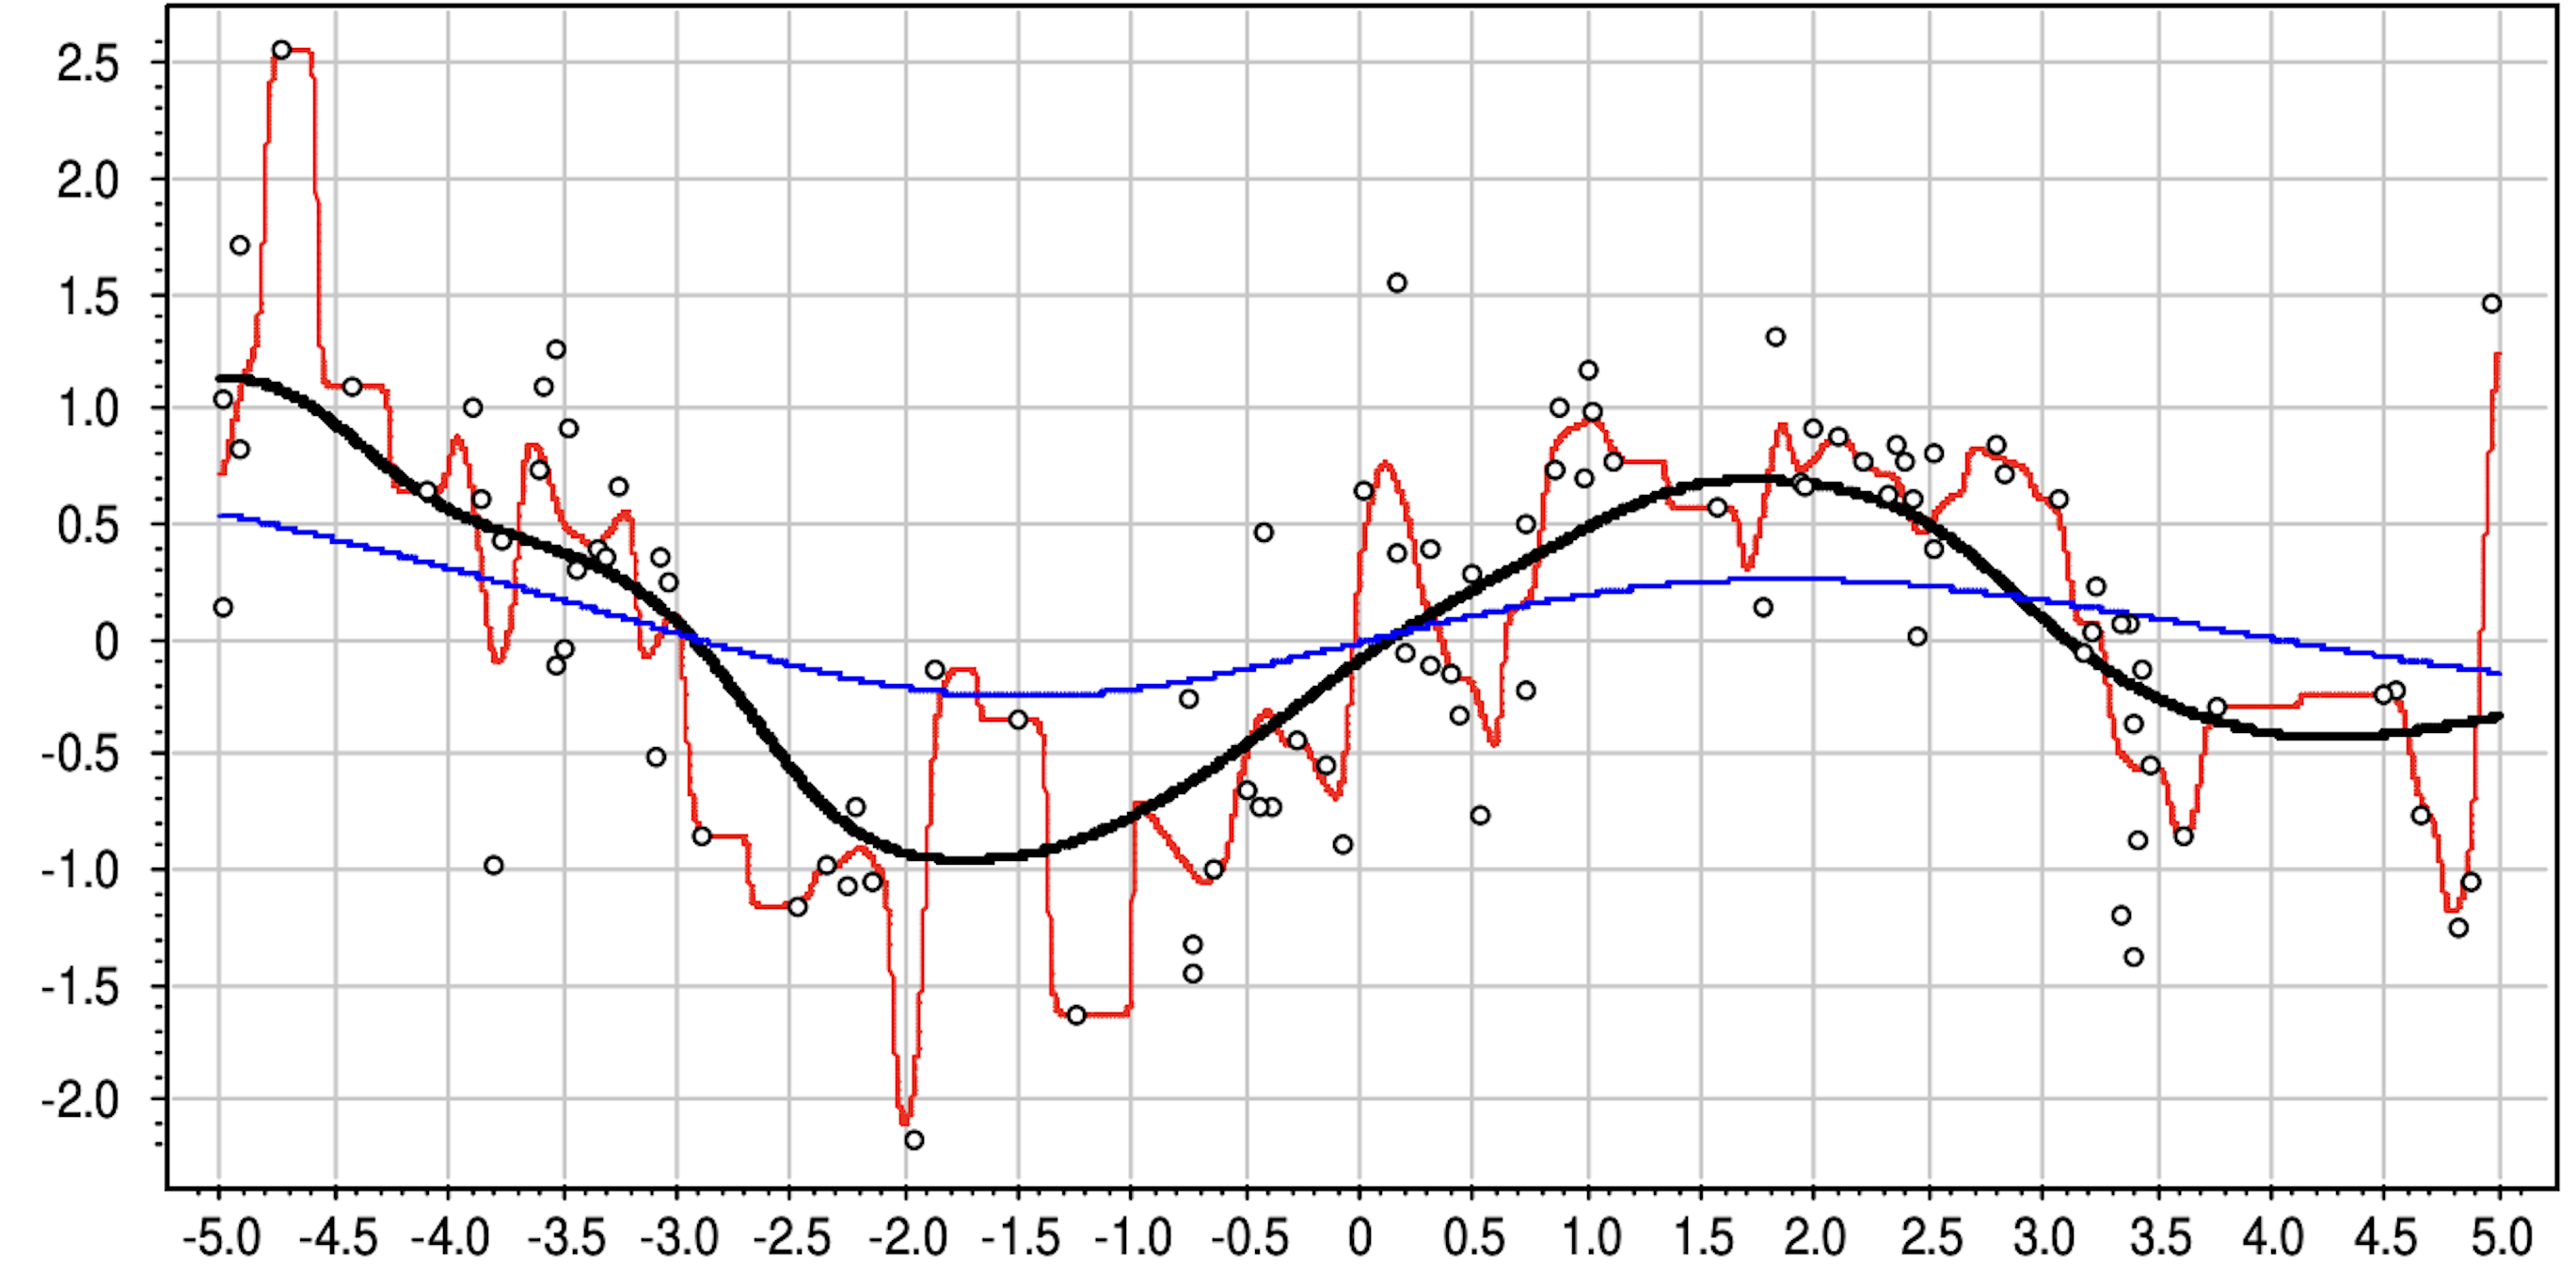
\includegraphics[width=\textwidth]{chapters/metric/images/I2.png}
    \label{fig:kernel_choice}
\end{align*}

\begin{itemize}
    \item Гауссовское ядро \(\Rightarrow\) гладкая аппроксимация
    \item Ширина окна существенно влияет на точность аппроксимации
\end{itemize}

\section*{Выбор ядра \(K\) и ширины окна \(h\)}

\noindent
\(h \in \{\textcolor{red}{0.1}, 1.0, \textcolor{blue}{3.0}\}\), треугольное ядро \(K(r) = (1 - \lvert r \rvert) [{\lvert r \rvert \leq 1}]\). Графики с разными значениями \(h\) при треугольном ядре:
\begin{align*}
    \centering
    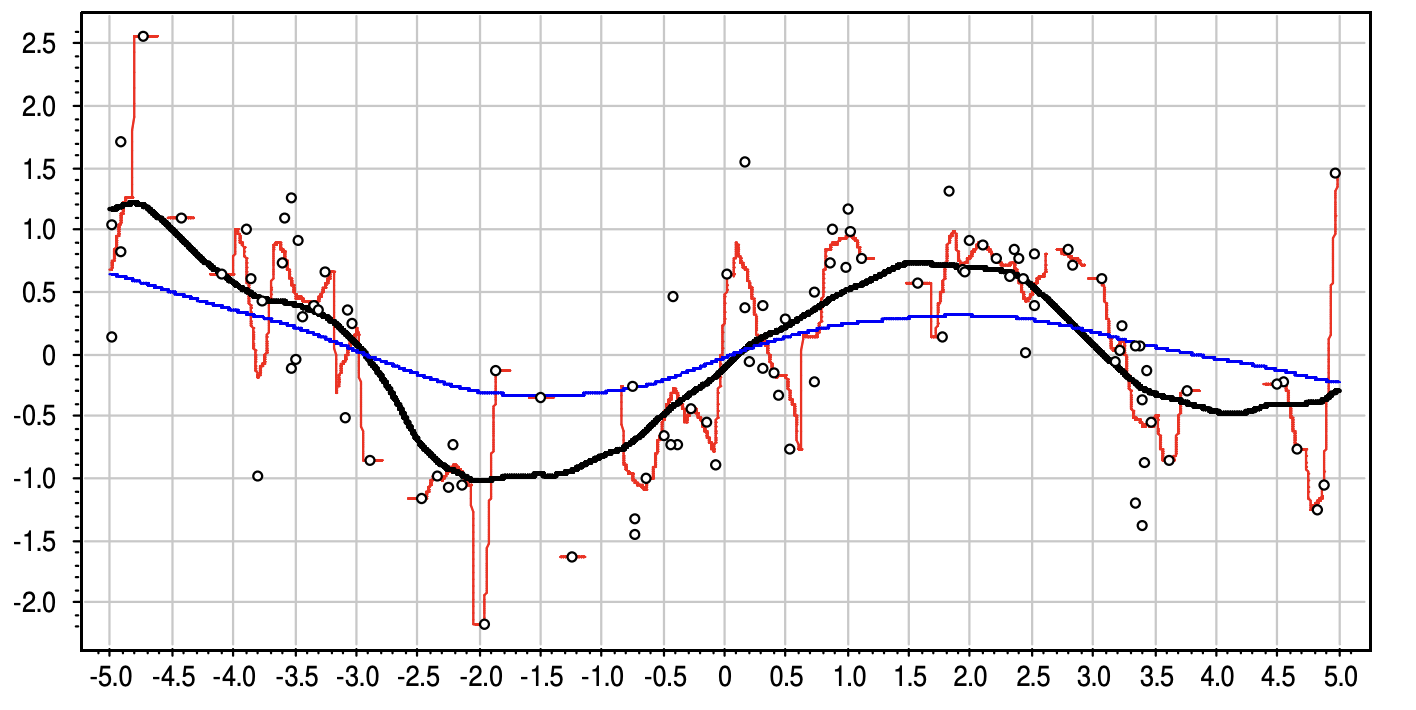
\includegraphics[width=\textwidth]{chapters/metric/images/I3.png}
    \label{fig:kernel_triangle}
\end{align*}

\begin{itemize}
    \item Треугольное ядро \(\Rightarrow\) кусочно-линейная аппроксимация
    \item Аппроксимация не определена, если в окне нет точек выборки
\end{itemize}

\section*{Выбор ядра \(K\) и ширины окна \(h\)}

\begin{itemize}
    \item \textbf{Ядро \(K(r)\)}
    \begin{itemize}
        \item существенно влияет на гладкость функции \( a_h(x) \),
        \item слабо влияет на качество аппроксимации.
    \end{itemize}
    \item \textbf{Ширина окна \(h\)}
    \begin{itemize}
        \item существенно влияет на качество аппроксимации.
    \end{itemize}
    \item \textbf{Переменная ширина окна по \(k\) ближайшим соседям:}
    \[
    w_i(x) = K\left( \frac{\rho(x, x_i)}{h(x)} \right), \quad h(x) = \rho(x, x^{(k+1)})
    \]
    где \(x^{(k)}\) — \(k\)-й сосед объекта \(x\).

    \item \textbf{Оптимизация ширины окна по скользящему контролю:}
    \[
    \text{LOO}(h, X^\ell) = \sum_{i=1}^\ell \left( a_h(x_i; X^\ell \setminus \{x_i\}) - y_i \right)^2 \to \min_h
    \]
\end{itemize}

\section*{Проблема выбросов (эксперимент на синтетических данных)}

\noindent
\(\ell = 100\), \(h = 1.0\), гауссовское ядро \(K(r) = \exp(-2r^2)\)

\vspace{0.5em}

{\color{red}Две из 100 точек — выбросы с ординатами \(y_i = 40\) и \(-40\)}

\vspace{0.5em}

{\color{blue}Синяя кривая — выбросов нет}

\begin{align*}
    \centering
    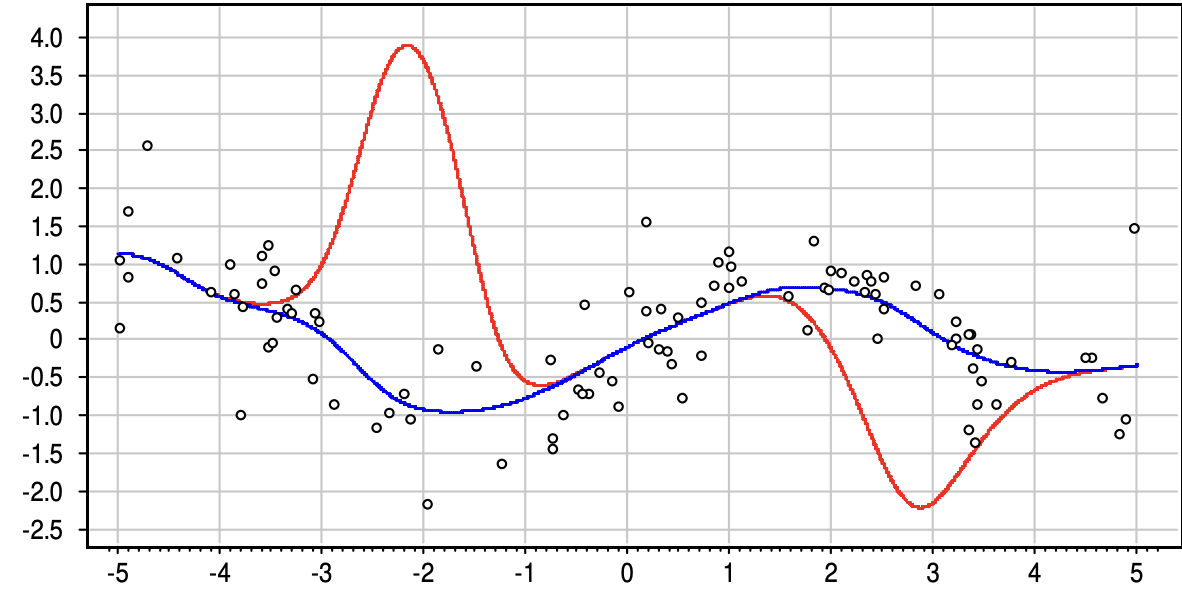
\includegraphics[width=\textwidth]{chapters/metric/images/I4.png}
    \label{fig:kernel_triangle}
\end{align*}

\section*{Проблема выбросов и локально взвешенное сглаживание}

\textbf{Проблема выбросов:} точки с большими случайными ошибками \(y_i\) сильно искажают функцию \(a_h(x)\)

\vspace{1em}
\textbf{Основная идея:} \\
чем больше величина ошибки \(\varepsilon_i = \lvert a_h(x_i; X^\ell \setminus \{x_i\}) - y_i \rvert\), \\
тем больше прецедент \((x_i, y_i)\) похож на выброс, \\
тем меньше должен быть его вес \(w_i(x)\).

\vspace{1em}
\textbf{Эвристика:} \\
домножить веса \(w_i(x)\) на коэффициенты \(\gamma_i = \tilde{K}(\varepsilon_i)\), \\
где \(\tilde{K}\) — ещё одно ядро, вообще говоря, отличное от \(K(r)\).

\vspace{1em}
\textbf{Рекомендация:} \\
квартическое ядро \(\tilde{K}(\varepsilon) = K_Q \left( \frac{\varepsilon}{6 \, \mathrm{med}\{\varepsilon_i\}} \right)\), \\
где \(\mathrm{med}\{\varepsilon_i\}\) — медиана вариационного ряда ошибок.

\section*{Алгоритм LOWESS (LOcally WEighted Scatter plot Smoothing)}

\vspace{1em}
\textcolor{blue}{\textbf{Вход:}} \(X^\ell\) — обучающая выборка; \\
\textcolor{blue}{\textbf{Выход:}} коэффициенты \(\gamma_i, \quad i = 1, \ldots, \ell\);

\vspace{1em}
инициализация: \(\gamma_i := 1, \quad i = 1, \ldots, \ell\);

\vspace{1em}
\textcolor{blue}{\textbf{повторять}}
\begin{itemize}
    \item оценки скользящего контроля в каждом объекте:
    \[
    a_i := a_h(x_i; X^\ell \setminus \{x_i\}) = \frac{\sum\limits_{j=1, j \neq i}^{\ell} y_j \gamma_j K\left( \frac{\rho(x_i, x_j)}{h(x_i)} \right)}{\sum\limits_{j=1, j \neq i}^{\ell} \gamma_j K\left( \frac{\rho(x_i, x_j)}{h(x_i)} \right)}, \quad i = 1, \ldots, \ell;
    \]
    \item \(\gamma_i := \tilde{K}(\lvert a_i - y_i \rvert), \quad i = 1, \ldots, \ell;\)
\end{itemize}

\textcolor{blue}{\textbf{пока}} коэффициенты \(\gamma_i\) не стабилизируются;

\section*{Пример работы LOWESS на синтетических данных}

\noindent
\(\ell = 100\), \(h = 1.0\), гауссовское ядро \(K(r) = \exp(-2r^2)\)

\vspace{1em}

Две из 100 точек — выбросы с ординатами \(y_i = 40\) и \(-40\)

\vspace{1em}

В данном случае LOWESS сходится за несколько итераций:
\begin{align*}
    \centering
    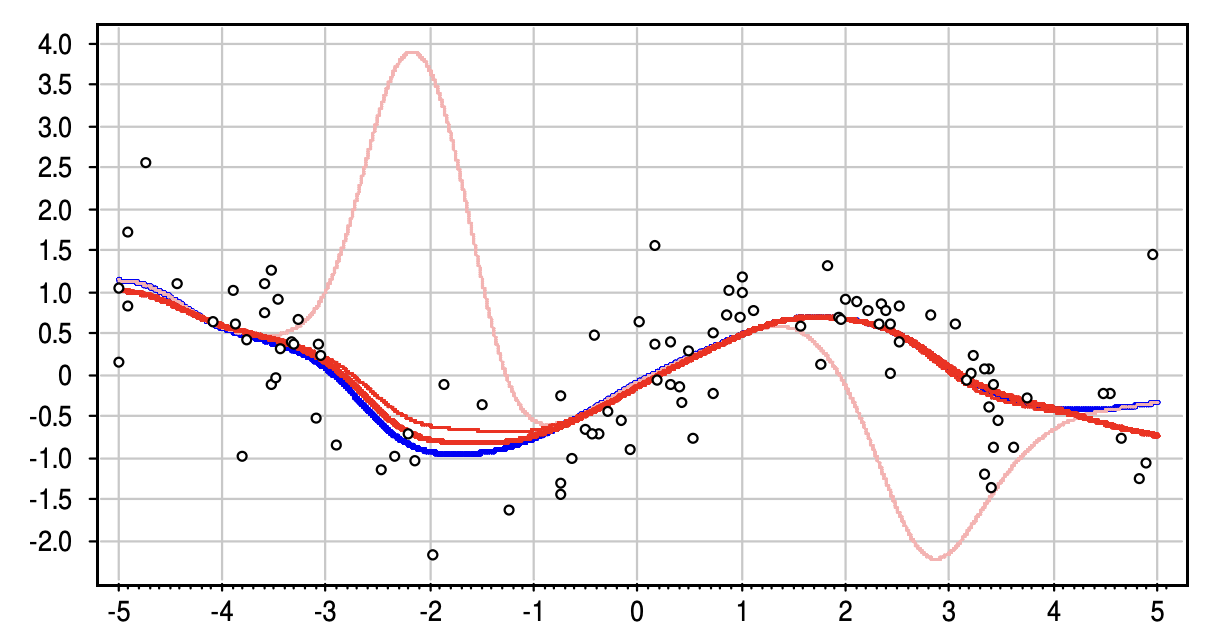
\includegraphics[width=\textwidth]{chapters/metric/images/I5.png}
    \label{fig:kernel_triangle}
\end{align*}

\section{Задачи}
\subsection{Задача 1}
Объясните, как выбор ядра \(K(r)\) влияет на гладкость регрессионной функции \(a_h(x)\). Приведите примеры различных ядер и их влияния.
\subsection{Ответ:}
Ядро \(K(r)\) определяет форму и вес окрестности точки, используемой для оценки регрессионной функции. Гладкие ядра, такие как гауссовское, дают более плавные оценки, в то время как менее гладкие, такие как прямоугольное, приводят к менее сглаженным функциям. Например:

- Гауссовское ядро \(K(r) = \exp(-r^2)\) — даёт плавные, гладкие оценки.

- Треугольное ядро \(K(r) = 1 - \lvert r \rvert\) (при \(\lvert r \rvert \leq 1\)) — более резкое, но все ещё гладкое.

- Прямоугольное ядро \(K(r) = 0.5\) (при \(\lvert r \rvert \leq 1\)) — приводит к кусочно-постоянной функции.

\subsection{Задача 2}
Приведите пример оптимального веса \(w_i(x)\) в алгоритме LOWESS, если известно распределение ошибок в данных. Поясните, как это распределение должно влиять на выбор веса, и почему весовое ядро \(\tilde{K}\) должно учитывать распределение ошибок.

\subsection{Ответ:}
Если ошибка \(\varepsilon_i\) распределена согласно некоторому известному распределению, например нормальному, \( \varepsilon_i \sim \mathcal{N}(0, \sigma^2)\), то весовой коэффициент должен минимизировать дисперсию предсказания. Весовая функция \(\tilde{K}(\varepsilon_i)\) должна убывать, когда \(\varepsilon_i\) отклоняется от некоторого центрального значения (0 для нормального распределения), чтобы уменьшить влияние выбросов:

\[
w_i(x) = \exp\left(-\frac{\varepsilon_i^2}{2\sigma^2}\right)
\]

Этот вес сильнее подавляет ошибки, отклоняющиеся от средней, что уменьшает их влияние на итоговую модель. Выбор весового ядра \(\tilde{K}\) должен учитывать распределение ошибок, чтобы учесть типичные вариации данных.

\subsection{Задача 3}
На основе метода LOWESS предложите способ оценки доверительного интервала для предсказаний. Выведите формулу для доверительного интервала и объясните, как она может быть использована для оценки надежности модели.

\subsection{Ответ:}

\quad 1. Построение модели:

   - Применим LOWESS для построения основной модели, получив предсказанные значения \( \hat{y}_i \) для каждого \(x_i\).

2. Оценка остаточной дисперсии:

   - Вычислим остаточные отклонения \(e_i = y_i - \hat{y}_i\).
   
   - Оценим дисперсию ошибок \(\sigma^2\) как среднеквадратическое отклонение:

     \[
     \sigma^2 = \frac{1}{n-k} \sum_{i=1}^{n} e_i^2
     \]

   где \(n\) — число точек данных, \(k\) — число параметров (в случае LOWESS, это скорее степень полинома в локальных регрессиях).

3. Построение доверительного интервала:

   - Для каждого предсказанного значения \( \hat{y}_i \) построим доверительный интервал, используя стандартное отклонение остаточных ошибок и критические значения из t-распределения:

     \[
     \hat{y}_i \pm t_{\alpha/2, n-k} \cdot \sqrt{\frac{\sigma^2}{n_i}}
     \]

   где \( t_{\alpha/2, n-k} \) — квантиль t-распределения с уровнем значимости \(\alpha\), и \(n_i\) — эффективное число точек в окрестности \(x_i\) (окрестность, которая использовалась для регрессии, может быть выражена размером окна или числом соседей).

4. Использование доверительных интервалов:

   - Доверительные интервалы позволяют пользователю оценить, насколько "надёжны" предсказанные значения. Узкие интервалы свидетельствуют о высокой уверенности.
   
   - Визуализация доверительных интервалов на графиках помогает выявлять области, где модель может быть неопределённой или подверженной ошибкам.

\section{Формула Надарая-Ватсона.}
 $X$ -объекты
 $Y$ -ответы 
 $X = (x_i, y_i)^l_{i=1}$-обучающая выборка
Будем обозначать $x_i = (x_i^1, ..., x_i^n)$ - вектор признаков объекта $x_i$. 

$a(x)= f(x,\theta)$ - параметрическая модель зависимости
$\theta$ -вектор параметров модели

Метод наименьших квадратов (МНК):
\begin{equation*}
    \displaystyle Q(\theta; X^l) =  \sum\limits_{i=1}^l(f(x_i, \theta)-y_i)^2w_i \longrightarrow \min_\theta, 
\end{equation*}
где $w(i,x)$ - некоторый вес, отражающий степень важности i-ого объекта. Вес неотрицателен и не возрастает по $i$. 


Сложно определить, какую стоит взять параметрическую модель.

\textit{Идея:}
Будем считать, что $f(x_i, \theta)=\theta$,  а $w_i$ зависит от x - т. е. веса объектов задаются в зависимости от того, на каком объекте будет получен объект.
Мы будем обучаться для каждого объекта, на котором хотим получить y. 

Тогда:
\begin{equation*}
    \displaystyle Q(\theta; X^l) =  \sum\limits_{i=1}^l(\theta-y_i)^2w(i,x) \longrightarrow \min_\theta, 
\end{equation*}
Наконец, положим
\begin{equation*}
    \displaystyle w_i(x) = K\left(\frac{\rho(x, x^{(i)})}{h}\right),
\end{equation*}
где $K(r)$ - невозрастающая функция, определённая на неотрицательных числах, называемая ядром, положительная на отркезке $[0,1]$, $h$ - ширина окна. То есть, чем больше расстояние до $x^{(i)}$, тем меньше оно влияет на x.
\\ Продифференцируем $Q(\theta; X^l)$ по $\theta$ и приравняем получившееся значение 0, и отсюда получим формулу ядерного сглаживания Надарая-Ватсона: 
\begin{equation*}
   \textcolor{blue} {\theta(x, X^l)= \frac{\sum\limits_{i=1}^ly_iw_i(x)}{\sum\limits_{i=1}^lw_i(x)}= \frac{\sum\limits_{i=1}^ly_iK\left(\frac{\rho(x, x^{(i)})}{h}\right)}{\sum\limits_{i=1}^lK\left(\frac{\rho(x, x^{(i)})}{h}\right)}}
\end{equation*}

Средневзвешенное значение y на тех объектах, которые близки к x.

Мы видим, что такой метод для каждого объекта $x$ рассматривает только объекты обучающей выборки, находящиеся на расстоянии не больше $h$ от $x$. Причём, чем дальше объект от $x$, тем  меньший вклад он даёт в оценку близости.



\textbf{Обоснование формулы Надарая-Ватсона:}

\textbf{Теорема:}
пусть выполнены следующие условия:
\begin{enumerate}
    \item Выборка $X^l$ простая из совместного распределения $p(x,y)$
    \item ядро $K(r)$ ограничено $\displaystyle\int\limits_{0}^{+\infty} K(r)dr < \infty$, 
    $\lim\limits_{r \to \infty}  rK(r) =0$.
    (из этого условия следует, что ядро приводит большие расстояния в 0)
    \item зависимость E(y|x) не имеет вертикальных асимптот
    
    $E(y^2|x)=\displaystyle\int\limits_{Y} y^2p(y|x)dy < \infty$ при любом $x \in X$
    \item последовательность $h_l$ (ширина окна) убывает с ростом выборки, но не слишком быстро и не слишком медленно
    $\lim\limits_{l\to \infty} h_l=0$,
    $\lim\limits_{l\to \infty} l h_l=0$
    
    Тогда имеет место сходимость по вероятности:
    $\theta(x, X^l) \xrightarrow{p}E(y|x) $

(здесь Е -мат. ожидание у при условии х)
    
    в любой точке $x \in X$, в которой E(y|x),  p(x), D(y|x) -непрерывны, p(x)>0
\end{enumerate}

По теореме даже если распределение $p(x,y)$ и E(y|x) не известны, $\theta$ будет стремится к нему с ростом длины обучающей выборки


\textit{Замечание.} Ширина окна отвечает за пере или недообучение,
следовательно сильно влияет на качество аппроксимации. 



Для подбора наилучшей модели оптимизируются параматры:
\begin{itemize}
    \item ширина окна $h$;
    \item ядро $K$. 
\end{itemize}

 Приведём примеры наиболее часто используемых ядер:
\begin{itemize}
    \item $\displaystyle K_1(r) = (1-r^2)[r\le1]$ - ядро Епанечникова;
    \item $\displaystyle K_2(r) = (1-r^2)^2[r\le1]$ - квартическое ядро;
    \item $\displaystyle K_3(r) = (1-|r|)[r\le1]$ - треугольное ядро; 
    \item $\displaystyle K_4(r) = [r\le1]$ - прямоугольное ядро; \item $\displaystyle K_5(r) = e^{-2r^2}$ - гауссовское ядро.
\end{itemize}
\textit{Замечание.} Существует проблема выбросов, при которой точки с большими случайными $y_i$ сильно искажают итоговую функцию. С этим можно справиться, домножив веса $w_i$ на коэффициенты $\gamma_i = K^*(\epsilon_i)$, где $\epsilon_i =|\theta(x_i, X^l)-y_i|$ подразумевается, что из $X^l$ исключили $x_i, K^*$-другое ядро


\textbf{Задача 1.}
Объяснить, почему не стоит брать финитное ядро на неизвестных данных при малой ширине окна h. Объяснить, почему нельзя просто взять большое h, чтобы решить проблему из предыдущего пункта. 

\textbf{Ответ:} 
При малой ширине окна h и финитном ядре у некоторых точек может не оказаться соседей, попадающих в радиус ядра К. На случай такого события в формулу Надарая-Ватсона в знаменатель добавляют малый член, чтобы не делить на 0.

Если увеличить ширину окна h, то для всех точек с большей вероятностью смогут найтись соседи, но в таком случае точность аппроксимации ухудшится.
\\

\textbf{Задача 2.}  как ядро влияет на гладкость функции? Ответ обосновать.

\textbf{Ответ:} 
Будем считать, что ядро не обращается в 0. 
Вспомним, что функция, являющаяся результатом деления двух гладких функций, является гладкой.
Сумма гладких функций, умноженных на число- также гладкая функция 
Пусть ядро К - гладкое, тогда ${\sum\limits_{i=1}^ly_iK\left(\frac{\rho(x, x^{(i)})}{h}\right)}$ -гладкое, и функция 
$\frac{\sum\limits_{i=1}^ly_iK\left(\frac{\rho(x, x^{(i)})}{h}\right)}{\sum\limits_{i=1}^lK\left(\frac{\rho(x, x^{(i)})}{h}\right)}$ 
будет гладкой

Следовательно, выбор ядра сильно влияет на гладкость.

\textbf{Задача 3.} Имеются следующие данные: x = [1.2, 2.7, 3.1, 4.5, 5.3],  y = [3.5, 1.8, 5.2, 2.1, 4.7].  Необходимо предсказать значение y для x = 2.5, используя формулу Надарая-Ватсона с квартическим ядром и h = 1.


\textbf{Решение:} Для каждой точки из набора данных вычисляем вес $K(\frac{x-x_i}{h})$, 

где x = 2.5, h =1,
Суммируем все вычисленные веса и делим каждый вес на эту сумму, чтобы получить нормированные веса.

веса не равны 0 только у точек x=2.7 x=3.1, их веса равны соответственно 0.9216 и 0.4096. 

При нормировке получим веса 0.6923 и 0.3077
Предсказание ŷ(2.5) вычисляется как взвешенная сумма значений по уже известной формуле 

примерный ŷ(2.5) =2.85


\section{Влияние выбора метрики на качество работы kNN}

Метод \(k\)-ближайших соседей (kNN) является одним из базовых алгоритмов машинного обучения и широко применяется в задачах классификации и регрессии. Этот алгоритм относится к метрическим методам, так как выбор ближайших соседей основывается на измерении расстояний между объектами. Главным фактором, определяющим качество модели, является выбор метрики расстояния, так как она определяет, какие объекты считаются «похожими».

\subsection{Сущность метода \(k\)-ближайших соседей}

Алгоритм \(k\)-ближайших соседей работает следующим образом:
\begin{enumerate}
    \item Для нового объекта вычисляется расстояние до всех объектов обучающей выборки.
    \item Выбираются \(k\) ближайших объектов в соответствии с выбранной метрикой.
    \item Класс нового объекта определяется на основе классов выбранных соседей (например, по принципу большинства для задач классификации).
    \item В задачах регрессии целевое значение нового объекта вычисляется как среднее (или взвешенное среднее) значений соседей.
\end{enumerate}

Ключевым аспектом метода является расстояние, вычисляемое на основе метрики, которая влияет на работу алгоритма, в том числе на точность и устойчивость модели.

\subsection{Популярные метрики расстояния}

\begin{enumerate}
    \item \textbf{Евклидова метрика} (\(L2\)-норма):  
    Одна из самых популярных метрик, измеряющая геометрическое расстояние между точками в пространстве.  
    Формула:
    \[
    d(x, y) = \sqrt{\sum_{i=1}^{n}(x_i - y_i)^2}
    \]
    Особенности:
    \begin{itemize}
        \item Подходит для данных, где все признаки одинаково масштабированы.
        \item Чувствительна к выбросам, так как квадрат отклонения значительно увеличивает вклад большого расхождения.
    \end{itemize}

    \item \textbf{Манхэттенская метрика} (\(L1\)-норма):  
    Измеряет расстояние как сумму абсолютных разностей координат.  
    Формула:
    \[
    d(x, y) = \sum_{i=1}^{n}|x_i - y_i|
    \]
    Особенности:
    \begin{itemize}
        \item Лучше подходит для разреженных данных.
        \item Менее чувствительна к выбросам по сравнению с Евклидовой метрикой.
    \end{itemize}

    \item \textbf{Метрика Минковского}:  
    Обобщение Евклидовой и Манхэттенской метрик.  
    Формула:
    \[
    d(x, y) = \left(\sum_{i=1}^{n}|x_i - y_i|^p\right)^{\frac{1}{p}}
    \]
    Особенности:
    \begin{itemize}
        \item При \(p=2\) совпадает с Евклидовой метрикой, при \(p=1\) — с Манхэттенской.
        \item Позволяет гибко настраивать степень влияния больших отклонений через параметр \(p\).
    \end{itemize}

    \item \textbf{Косинусное расстояние}:  
    Измеряет угол между векторами, игнорируя их длину.  
    Формула:
    \[
    d(x, y) = 1 - \frac{\langle x, y \rangle}{\|x\| \cdot \|y\|}
    \]
    Особенности:
    \begin{itemize}
        \item Часто применяется для текстовых данных (например, векторов TF-IDF).
        \item Устойчиво к изменениям масштаба векторов.
    \end{itemize}

    \item \textbf{Метрика Чебышёва}:  
    Учитывает максимальное различие по одной из координат.  
    Формула:
    \[
    d(x, y) = \max_{i}|x_i - y_i|
    \]
    Особенности:
    \begin{itemize}
        \item Удобна для задач, где критически важно учитывать наибольшее расхождение.
        \item Формирует кубические границы ближайших соседей.
    \end{itemize}
\end{enumerate}

\subsection{Влияние выбора метрики на качество работы модели}

Выбор метрики может значительно изменить поведение алгоритма \(k\)-ближайших соседей. Основные факторы влияния:

\begin{enumerate}
    \item \textbf{Геометрия данных:}  
    Разные метрики формируют разные границы классов. Например, Евклидова метрика создает округлые границы, а Манхэттенская — прямоугольные. В задачах с нелинейными разделяющими гиперплоскостями может потребоваться комбинированный подход или нестандартные метрики.

    \item \textbf{Масштаб признаков:}  
    Метрики, такие как Евклидова, чувствительны к различиям в масштабе признаков. Например, если один признак имеет диапазон [0, 1], а другой — [0, 1000], последний будет доминировать. Для решения этой проблемы применяется нормализация или стандартизация данных.

    \item \textbf{Шум и выбросы:}  
    Метрики по-разному реагируют на шум. Евклидова метрика чувствительна к выбросам, так как квадратичное расстояние значительно увеличивается для больших расхождений. Метрики, такие как Манхэттенская или косинусное расстояние, менее чувствительны к шуму.

    \item \textbf{Высокая размерность:}  
    В задачах с большим количеством признаков (проблема «проклятия размерности») расстояния между всеми объектами становятся примерно одинаковыми. Это снижает различимость ближайших соседей, что делает выбор метрики критически важным.

    \item \textbf{Специфика задачи:}  
    Например, для задач обработки текстов косинусная метрика часто оказывается лучше, так как она учитывает только направление векторов, игнорируя их длину. Для задач с пространственными данными чаще применяются Евклидова или Манхэттенская метрика.
\end{enumerate}

\subsection{Примеры задач}

\begin{enumerate}
    \item \textbf{Теоретическая задача:}  
    Рассмотрите два набора данных из двух классов, представленных точками на плоскости.  
    Постройте границы разделения классов при использовании:
    \begin{itemize}
        \item Евклидовой метрики,
        \item Манхэттенской метрики.
    \end{itemize}
    Объясните, как выбор метрики влияет на форму границ.

    \item \textbf{Практическая задача:}  
    Используя набор данных \texttt{Iris}, обучите модель \(k\)-ближайших соседей с Евклидовой, Манхэттенской и косинусной метриками. Сравните метрики качества (точность, F1-меру) и сделайте вывод о том, какая метрика работает лучше и почему.

    \item \textbf{Исследовательская задача:}  
    Для синтетических данных с перекрывающимися классами разработайте алгоритм выбора оптимальной метрики с использованием кросс-валидации. Постройте графики зависимости точности от параметра \(k\) для разных метрик.
\end{enumerate}

\subsection{Заключение}

Выбор метрики расстояния является ключевым фактором, определяющим качество работы метода \(k\)-ближайших соседей. Оптимальная метрика зависит от природы данных, задачи и требований к точности и устойчивости модели. Для улучшения результатов рекомендуется проводить предварительный анализ данных, нормализацию признаков и тестирование нескольких метрик с использованием кросс-валидации.
